\chapter{Design}

As the application is a web application the design of the user interface was very important.  The overall design implemented was designed to be straight forward to use and elegant in appearance as well as re-enforcing the overall theme of the application.  

\begin{figure}[H]
  \centering
    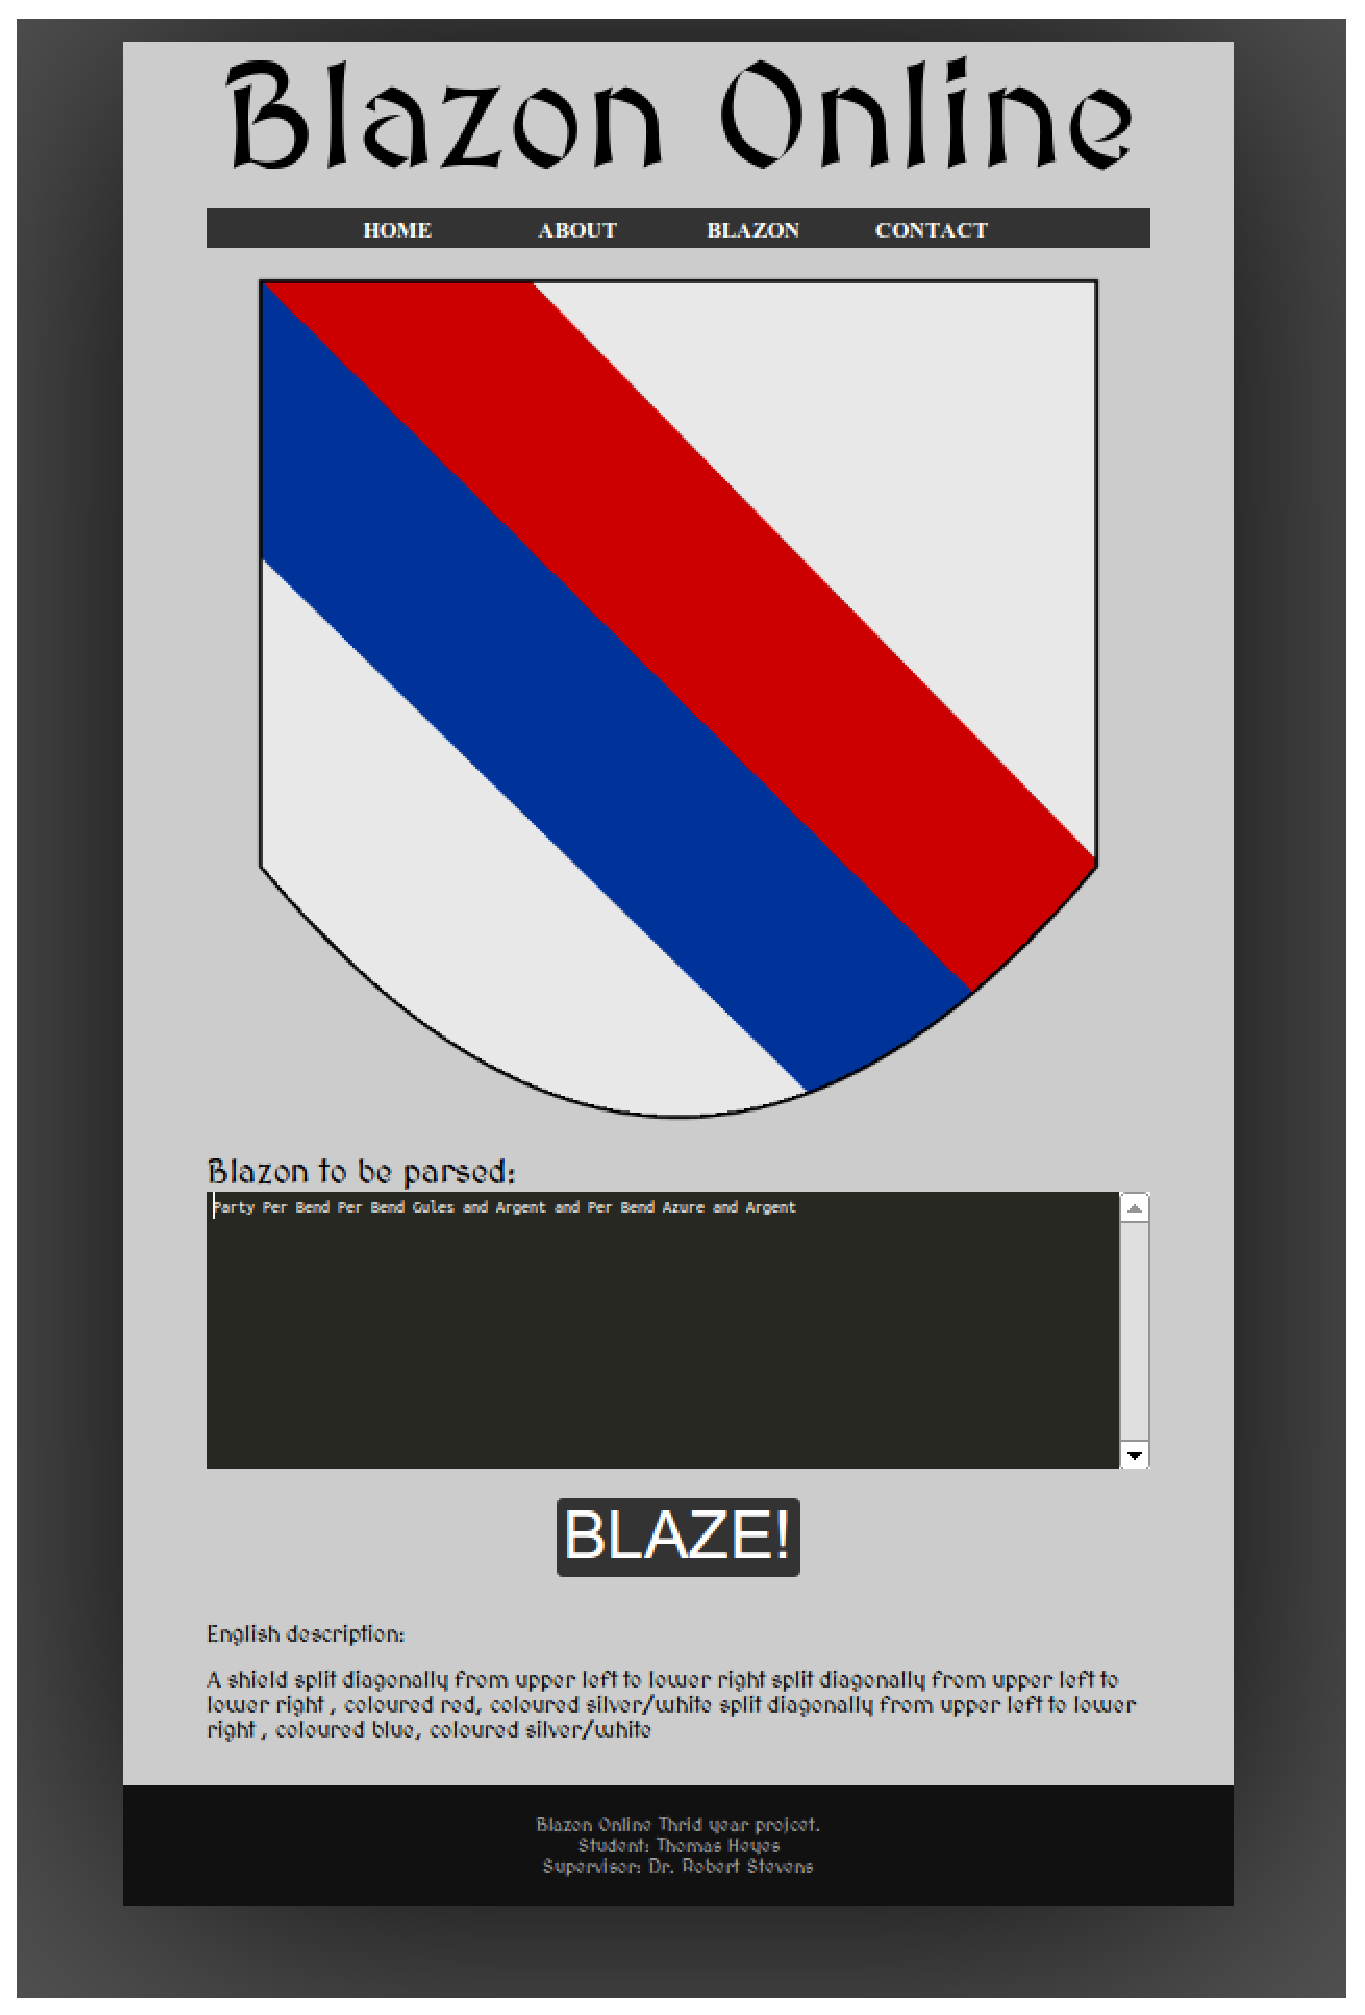
\includegraphics[width=\textwidth]{design/images/overall.eps}
  \caption{An overview of the user interface of the web application.}
  \label{fig:overall}
  
\end{figure}

\section{A Functional Layout}

The main body of the application consists of three components, the \emph{HTML5 Canvas} element onto which Shields are rendered, the text area into which the user inputs Blazon and the button the end user clicks  to initialize parsing of the input.


These three components are placed centrally and grouped together so a user assumes they are related to each other.  To illustrate that blazon goes into the text area an example sentence is pre-placed into it and parsed when the page is loaded.


\section{Feedback to the User}
Upon receiving erroneous input the application needs to inform the user that about why the sentence the application attempted to parse is invalid.  This was implemented using \emph{JavaScript} alerts because they open a window which is modal so that it holds the focus of the browser until acknowledged. 


\begin{figure}[H]
  \centering
    
\includegraphics[width=\textwidth]{design/images/error.eps}
  \caption{An overview of the user interface of the web application.}
  \label{fig:itsallgonewrong}
  
\end{figure}



\section{Maintaining the Blazon Theme}
As Blazon was prominent from the twelfth century onwards the font used for the static text on the application encompasses a medieval style.  Whilst only a 
minor detail it provides a complimenting style to the actual purpose and feel of the application.  The font is provided by \emph{Google}.\cite{font}. 

\begin{figure}[H]
  \centering
    
\includegraphics[width=\textwidth]{design/images/font.eps}
  \caption{An overview of the user interface of the web application.}
  \label{fig:yeoldfont}
\end{figure}

\section{The English Description}
The English description of the Blazon sentence is outputted below the three major components because the graphical representation of the shield is considerably more interesting for the user and contains almost as much detail. 

If a user particularly wants to view the English translation then it is in an obvious place but doesn't obscure or detract attention from the graphical version, which should be the more prominent. 


\section{Ace Editor} \label
The input area is more than just a standard HTML text area, it is an instance of the \emph{Ace Editor}\cite{Ace}. The \emph{Ace Editor} allows a text editor to be emended into a JavaScript application.  The original idea was to implement syntax highlighting for Blazon using the editor however this was not due to constraints on development time.











